% Metaphors.tex

\newpage 

\part{Metaphors and Analogies}



\begin{entry}
\heading{The Death Circle March}
\source{Army Ant Spiral of Death}
\date{May 1, 2016}

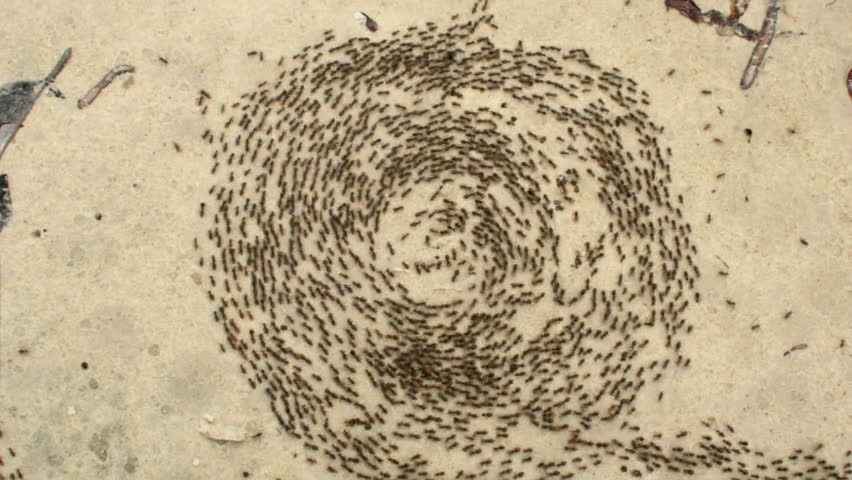
\includegraphics[width=.5\textwidth]{image/deathcircle}
\captionof{figure}{Blind army ants rely on the scent of other ants to navigate.  But sometimes they get stuck following each other into a circle without knowing that they are lost.  They eventally die as they diligently march on to what they think is the correct path.}

\background{
Warrior ants are blind and rely on the scent of other ants to navigate.  Sometimes they end up in what is called the death circle (get source or picture).  

Death Circle is like the apostasy.  A blind prophet cannot lead another blind man and both shall march in circles without hope until they die.
}

\end{entry}

\begin{entry}
\heading{Wear on Self-Worth}
\source{Tire Wear}
\background{Self actualization vs overinflated ego  and underinflated self worth}
\end{entry}


